% ============================================================
%  Geometric Observer Routing for Multi-View Graph Attention
%
%  Restructured Paper — March 2026
% ============================================================
\documentclass[11pt,a4paper]{article}

% ---------- packages ----------
\usepackage[margin=1in]{geometry}
\usepackage{amsmath,amssymb,amsthm,mathtools}
\usepackage{algorithm}
\usepackage{algpseudocode}
\usepackage{booktabs}
\usepackage{graphicx}
\usepackage{xcolor}
\usepackage{hyperref}
\usepackage{cleveref}
\usepackage{enumitem}
\usepackage{multirow}
\usepackage{caption}
\usepackage{subcaption}
\usepackage{natbib}
\usepackage{tikz}
\usetikzlibrary{positioning, arrows.meta, fit, backgrounds, calc, decorations.pathreplacing}

\graphicspath{{../../artifacts/figures/}}

\hypersetup{
  colorlinks=true,
  linkcolor=blue!70!black,
  citecolor=green!50!black,
  urlcolor=blue!60!black,
}

% ---------- theorem environments ----------
\newtheorem{theorem}{Theorem}
\newtheorem{proposition}[theorem]{Proposition}
\newtheorem{corollary}[theorem]{Corollary}
\newtheorem{lemma}[theorem]{Lemma}
\newtheorem{remark}{Remark}
\newtheorem{definition}{Definition}

% ---------- macros ----------
\newcommand{\ours}{\textsc{GoRA}}  % Geometric Observer-Routed Attention
\newcommand{\ourspp}{\textsc{GoRA++}}
\newcommand{\RR}{\mathbb{R}}
\newcommand{\EE}{\mathbb{E}}
\newcommand{\calM}{\mathcal{M}}
\newcommand{\calN}{\mathcal{N}}
\newcommand{\calL}{\mathcal{L}}
\newcommand{\bpi}{\boldsymbol{\pi}}
\newcommand{\boldA}{\mathbf{A}}
\DeclareMathOperator{\softmax}{softmax}
\DeclareMathOperator{\diag}{diag}

% ============================================================
\title{%
  Geometric Observer Routing for\\
  Multi-View Graph Attention}

\author{%
  Richard Liu\\
  University of North Carolina at Charlotte\\
  \texttt{wliu23@charlotte.edu}
}

\date{March 2026}

% ============================================================
\begin{document}
\maketitle

% ============================================================
%  ABSTRACT
% ============================================================
\begin{abstract}
When a graph admits multiple structural views---feature-based neighbors,
temporal proximity, spectral affinity---how should attention combine them?
We identify a fundamental \emph{isolation-versus-interaction tradeoff}:
mixing views \emph{before} the attention softmax enables cross-view
reinforcement but permits noisy views to dilute clean signals;
mixing \emph{after} preserves dominant-view fidelity but forfeits
cross-source synergy.
We prove that neither mode dominates and that the optimal choice is
predictable from measurable view properties (signal-to-noise ratio,
neighborhood overlap).

To exploit this tradeoff, we introduce \emph{geometric observer routing}
(\ours{}): an attention mechanism that routes heads to competing graph
views using manifold descriptors---curvature, intrinsic dimension,
density---rather than content features.
A log-barrier mask with learned per-head temperature provides a
differentiable relaxation of hard neighborhood constraints, yielding
end-to-end gradient flow from task loss through routing to view
selection.

On a controlled temporal-graph benchmark, isolation mode achieves
0.984~PR-AUC (+6.5 over GAT) when one view dominates; interaction mode
achieves 0.939~PR-AUC (+2.0 over GAT) when views are complementary.
Ablation confirms that geometric observers---especially curvature
($-7.5\%$ when removed)---carry routing signal that content features
cannot replace.
A practitioner's decision framework makes mode selection actionable.
\end{abstract}

% ============================================================
%  1. INTRODUCTION
% ============================================================
\section{Introduction}
\label{sec:intro}

Many real-world graph tasks admit multiple complementary structural
views of the same node set.
A fraud-detection system, for example, may construct a feature-similarity
graph connecting transactions with similar attributes, a temporal graph
linking transactions close in time, and a spectral graph capturing
diffusion patterns across the Laplacian.
Each view encodes distinct relational information, yet combining them
naively can \emph{degrade} performance---a phenomenon we trace to a
previously uncharacterized architectural tradeoff.

Graph attention networks \citep{velickovic2018graph, brody2022how}
extend transformer attention \citep{vaswani2017attention} to irregular
topologies but route information using only content-based query-key
similarity, with graph structure entering as a non-differentiable binary
mask.
Graph transformers \citep{ying2021transformers, rampasek2022recipe}
add structural encodings as fixed biases but do not learn
structure-aware routing.
Mixture-of-experts (MoE) architectures \citep{shazeer2017outrageously,
fedus2022switch} learn routing but gate on content alone, ignoring
manifold geometry.

None of these approaches address the central question: \emph{when
multiple graph views are available, how should an attention mechanism
combine them?}
We show that the answer depends on a fundamental
\textbf{isolation-versus-interaction tradeoff} that, to our knowledge,
has not been formally characterized in the multi-view attention
literature.

\paragraph{The tradeoff.}
Combining views \emph{before} the attention softmax (pre-softmax mixing)
forces all views' edges to compete for the same probability mass,
enabling cross-view reinforcement but allowing noisy views to dilute
clean signals.
Combining views \emph{after} the softmax (post-softmax mixing) computes
per-view attention independently and routes the outputs, preserving
dominant-view fidelity but sacrificing cross-view synergy.
Neither mode dominates across data regimes
(\Cref{sec:drift}): the optimal choice is predictable from the signal
structure of the available views.

\paragraph{Geometric descriptors as routing priors.}
To navigate this tradeoff, we propose routing attention heads using
geometric descriptors of local graph structure---curvature, intrinsic
dimension, and density---rather than content features.
These descriptors encode manifold geometry directly, providing an
\emph{inductive bias for view selection} analogous to how spatial
frequency filters in early vision extract geometric structure before
semantic processing.
We compute these descriptors in an \emph{observer layer} that informs
routing before any content-based attention occurs.

\paragraph{Contributions.}
\begin{enumerate}[label=(\arabic*),nosep]
  \item \textbf{Isolation-versus-interaction tradeoff.}
    We formalize a fundamental property of multi-view attention:
    combining views before versus after softmax normalization yields
    complementary inductive biases whose relative advantage is
    predictable from view signal-to-noise ratios and neighborhood
    overlap (\Cref{sec:tradeoff,sec:drift}).
  \item \textbf{Geometric observer routing.}
    We introduce an attention-routing mechanism driven by manifold
    descriptors (curvature, intrinsic dimension, density) rather than
    content features, and show empirically that curvature alone
    accounts for a 7.5\% performance gap
    (\Cref{sec:observers,sec:observer_analysis}).
  \item \textbf{Log-barrier differentiable masking.}
    We formalize a continuous relaxation of hard attention masks via a
    log-barrier with learned per-head temperature, enabling end-to-end
    gradient flow through the full routing chain
    (\Cref{sec:logbarrier}).
  \item \textbf{Practitioner's decision framework.}
    We provide measurable criteria for selecting the optimal attention
    mode, making the tradeoff actionable for deployment
    (\Cref{sec:guide}).
\end{enumerate}
We additionally explore extensions---view-specific projections and a
scalable alignment proxy---reporting both positive and negative results
honestly (\Cref{sec:thornpp_eval}).


% ============================================================
%  2. THE ISOLATION-INTERACTION TRADEOFF
% ============================================================
\section{The Isolation-Interaction Tradeoff}
\label{sec:tradeoff}

Before describing our architecture, we formalize the core theoretical
observation that motivates it.
This tradeoff applies to any multi-source attention system, not only
graphs.

\subsection{Setup}
\label{sec:tradeoff_setup}

Let $\calN^{(m)}(i)$ denote the neighborhood of node $i$ in view $m$,
and $\calN_\cup(i) = \bigcup_m \calN^{(m)}(i)$ the union neighborhood.
Define $\rho_i = |\bigcap_m \calN^{(m)}(i)| / |\calN_\cup(i)|$ as the
\emph{view overlap ratio} and $\mathrm{SNR}_m$ as the signal-to-noise
ratio of view $m$ (ratio of signal-feature variance to noise-feature
variance within $\calN^{(m)}(i)$).
Let $s_{ij}^{(h)}$ be the content-based attention score and
$\pi_{i,h,m}$ the routing weight assigned to view $m$ by head $h$ at
node $i$.

\subsection{Two Mixing Modes}
\label{sec:two_modes}

\paragraph{Pre-softmax (interaction mode).}
Views are combined before the softmax, and a single normalization
covers the union neighborhood:
\begin{equation}
  \label{eq:pre_general}
  \alpha_{ij}^{(h)} = \softmax_{j \in \calN_\cup(i)}\!\Big(
    s_{ij}^{(h)} + f\!\big(\textstyle\sum_m \pi_{i,h,m} A_{ij}^{(m)}\big)
  \Big),
  \quad
  y_i^{(h)} = \sum_{j \in \calN_\cup(i)} \alpha_{ij}^{(h)} v_j^{(h)}.
\end{equation}
An edge $(i,j)$ appearing in multiple views accumulates weight from
each, enabling \emph{cross-view reinforcement}.
However, all views compete for the same probability mass: a noisy view
with many edges can dilute the attention assigned to a cleaner, sparser
view.

\paragraph{Post-softmax (isolation mode).}
Each view computes its own attention independently; routing combines
the outputs:
\begin{equation}
  \label{eq:post_general}
  \alpha_{ij}^{(h,m)} = \softmax_{j \in \calN^{(m)}(i)}\!
    \big(s_{ij}^{(h)}\big),
  \quad
  y_i^{(h)} = \sum_m \pi_{i,h,m}
    \sum_{j \in \calN^{(m)}(i)} \alpha_{ij}^{(h,m)} v_j^{(h)}.
\end{equation}
Each view's softmax normalizes only over its own neighborhood.
The dominant view's signal flows at full fidelity, and noisy views are
multiplicatively suppressed via low $\pi_{i,h,m}$.
However, the model cannot discover that edges present in multiple views
are more trustworthy.

\subsection{When Each Mode Dominates}
\label{sec:when_dominates}

The relative advantage of each mode follows from the view-quality
structure:

\begin{proposition}[Mode selection]
  \label{prop:mode_selection}
  Let $\mathrm{SNR}_m$ denote the signal-to-noise ratio of view $m$
  and $\rho_i$ the overlap ratio at node $i$.
  \begin{enumerate}[label=(\roman*),nosep]
    \item \textbf{Isolation dominates} when
      $\max_m \mathrm{SNR}_m \gg \mathrm{SNR}_{m'}$ for $m' \neq m$:
      post-softmax preserves the dominant view's clean attention while
      multiplicatively suppressing noisy views via
      $\pi_{i,h,m'} \approx 0$.
      Pre-softmax cannot fully suppress residual edges from noisy views
      because they share the union softmax normalization.
    \item \textbf{Interaction dominates} when $\rho_i$ is high and
      $\mathrm{SNR}_m$ values are comparable:
      pre-softmax enables cross-view reinforcement through
      $f(\sum_m \pi_m A^{(m)}_{ij}) > \max_m f(\pi_m A^{(m)}_{ij})$
      for shared edges.
      Post-softmax treats each view independently, missing this synergy.
  \end{enumerate}
\end{proposition}

This characterization is validated empirically in \Cref{sec:drift}
and yields the practitioner's decision framework in \Cref{sec:guide}.
The key insight is that \textbf{the optimal mode is a property of the
data, not the architecture}.


% ============================================================
%  3. ARCHITECTURE: OBSERVER-ROUTED MULTI-VIEW ATTENTION
% ============================================================
\section{Observer-Routed Multi-View Attention}
\label{sec:arch}

We now present \ours{} (\textbf{G}eometric \textbf{O}bserver-\textbf{R}outed
\textbf{A}ttention), which operationalizes the isolation-interaction
tradeoff through geometric observer routing.
\Cref{fig:architecture} provides a high-level overview.

\begin{figure}[t]
\centering
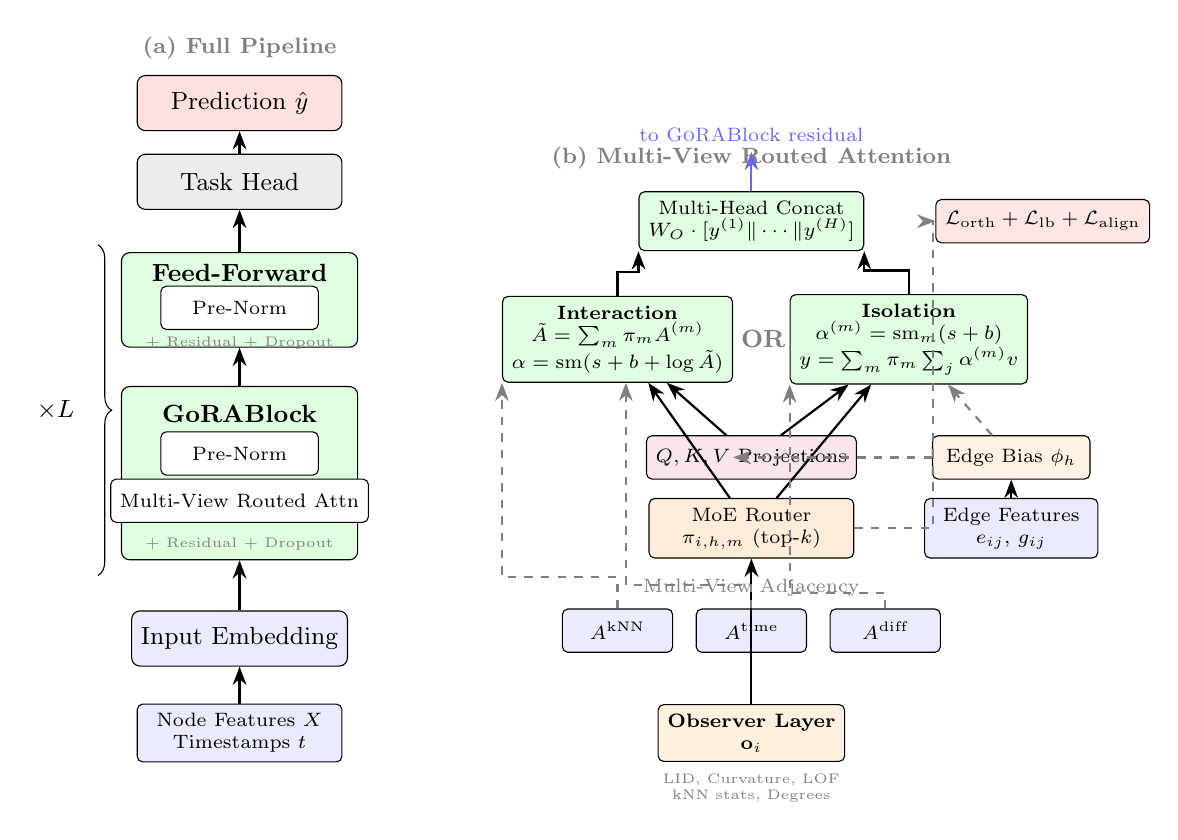
\begin{tikzpicture}[
  >=Stealth,
  block/.style={draw, rounded corners=3pt, minimum width=2.6cm,
    minimum height=0.7cm, align=center, font=\small},
  smallblock/.style={draw, rounded corners=2pt, minimum width=2.0cm,
    minimum height=0.55cm, align=center, font=\scriptsize},
  databox/.style={draw, rounded corners=2pt, fill=blue!8,
    minimum width=2.6cm, minimum height=0.55cm, align=center,
    font=\scriptsize},
  routerbox/.style={draw, rounded corners=2pt, fill=orange!15,
    minimum width=2.0cm, minimum height=0.55cm, align=center,
    font=\scriptsize},
  attnbox/.style={draw, rounded corners=2pt, fill=green!12,
    minimum width=2.0cm, minimum height=0.55cm, align=center,
    font=\scriptsize},
  lossbox/.style={draw, rounded corners=2pt, fill=red!10,
    minimum width=2.0cm, minimum height=0.55cm, align=center,
    font=\scriptsize},
  arrow/.style={->, thick},
  darrow/.style={->, thick, dashed, gray},
  brace/.style={decorate, decoration={brace, amplitude=5pt, mirror}},
]

% ===== LEFT COLUMN: Full Pipeline =====
\node[databox] (input) at (0, 0) {Node Features $X$\\Timestamps $t$};
\node[block, fill=blue!8] (embed) at (0, 1.2) {Input Embedding};

% GoRA Block x L
\node[block, fill=green!12, minimum height=2.2cm, minimum width=3.0cm]
  (gorablock) at (0, 3.3) {};
\node[font=\small\bfseries] at (0, 4.05) {\ours{}Block};
\node[smallblock, fill=white] (prenorm1) at (0, 3.55) {Pre-Norm};
\node[smallblock, fill=white] (mhra) at (0, 2.95) {Multi-View Routed Attn};
\node[font=\tiny, gray] at (0, 2.4) {+ Residual + Dropout};

\node[block, fill=green!12, minimum height=1.2cm, minimum width=3.0cm]
  (ffnblock) at (0, 5.5) {};
\node[font=\small\bfseries] at (0, 5.85) {Feed-Forward};
\node[smallblock, fill=white] (prenorm2) at (0, 5.4) {Pre-Norm};
\node[font=\tiny, gray] at (0, 4.95) {+ Residual + Dropout};

% Nx bracket
\draw[brace] (-1.8, 2.0) -- (-1.8, 6.2)
  node[midway, left=5pt, font=\small] {$\times L$};

\node[block, fill=gray!15] (taskhead) at (0, 7.0) {Task Head};
\node[block, fill=red!12] (output) at (0, 8.0) {Prediction $\hat{y}$};

% Arrows left column
\draw[arrow] (input) -- (embed);
\draw[arrow] (embed) -- (gorablock.south);
\draw[arrow] (gorablock.north) -- (ffnblock.south);
\draw[arrow] (ffnblock.north) -- (taskhead);
\draw[arrow] (taskhead) -- (output);

% ===== RIGHT COLUMN: Inside Routed Attention =====
% Observer features (the perception layer)
\node[databox, minimum width=2.2cm, fill=orange!12] (obs) at (6.5, 0.0)
  {\textbf{Observer Layer}\\$\mathbf{o}_i$};
\node[font=\tiny, gray, text width=2.5cm, align=center] at (6.5, -0.7)
  {LID, Curvature, LOF\\kNN stats, Degrees};

% Views
\node[databox, minimum width=1.4cm] (vknn) at (4.8, 1.3) {$A^{\text{kNN}}$};
\node[databox, minimum width=1.4cm] (vtime) at (6.5, 1.3) {$A^{\text{time}}$};
\node[databox, minimum width=1.4cm] (vdiff) at (8.2, 1.3) {$A^{\text{diff}}$};
\node[font=\scriptsize, gray] at (6.5, 1.85) {Multi-View Adjacency};

% Router
\node[routerbox, minimum width=2.6cm] (router) at (6.5, 2.6)
  {MoE Router\\$\pi_{i,h,m}$ (top-$k$)};
\draw[arrow] (obs) -- (router);

% Edge bias
\node[databox, minimum width=2.2cm] (edgefeat) at (9.8, 2.6)
  {Edge Features\\$e_{ij}$, $g_{ij}$};
\node[smallblock, fill=orange!10] (edgebias) at (9.8, 3.5)
  {Edge Bias $\phi_h$};
\draw[arrow] (edgefeat) -- (edgebias);

% Q, K, V
\node[smallblock, fill=purple!10, minimum width=2.6cm] (qkv) at (6.5, 3.5)
  {$Q, K, V$ Projections};

% Pre-softmax path
\node[attnbox, minimum width=2.6cm, minimum height=1.0cm] (presm)
  at (4.8, 5.0) {\textbf{Interaction}\\$\tilde{A} = \sum_m \pi_m A^{(m)}$\\
  $\alpha = \text{sm}(s + b + \log \tilde{A})$};

% Post-softmax path
\node[attnbox, minimum width=2.6cm, minimum height=1.0cm] (postsm)
  at (8.5, 5.0) {\textbf{Isolation}\\$\alpha^{(m)} = \text{sm}_m(s + b)$\\
  $y = \sum_m \pi_m \sum_j \alpha^{(m)} v$};

% Routing arrows to attention modes
\draw[arrow] (router) -- (presm);
\draw[arrow] (router) -- (postsm);
\draw[arrow] (qkv) -- (presm);
\draw[arrow] (qkv) -- (postsm);
\draw[darrow] (edgebias) -- (presm.east |- edgebias);
\draw[darrow] (edgebias) -- (postsm);

% View arrows to attention
\draw[darrow] (vknn.north) -- ++(0, 0.4) -| (presm.south west);
\draw[darrow] (vtime.north) -- ++(0, 0.3) -| ([xshift=3pt]presm.south);
\draw[darrow] (vdiff.north) -- ++(0, 0.2) -| (postsm.south west);

% OR node
\node[font=\small\bfseries, gray] at (6.65, 5.0) {OR};

% Output aggregation
\node[attnbox, minimum width=2.6cm] (agg) at (6.5, 6.5)
  {Multi-Head Concat\\$W_O \cdot [y^{(1)} \| \cdots \| y^{(H)}]$};
\draw[arrow] (presm.north) -- ++(0, 0.3) -| (agg.south west);
\draw[arrow] (postsm.north) -- ++(0, 0.3) -| (agg.south east);

% Regularizers
\node[lossbox, minimum width=2.4cm] (regs) at (10.2, 6.5)
  {$\calL_{\text{orth}} + \calL_{\text{lb}} + \calL_{\text{align}}$};
\draw[darrow] (router.east) -- ++(1.0, 0) |- (regs);

% Connection arrow from right to left
\draw[arrow, blue!60, thick] (agg.north) -- ++(0, 0.5)
  node[above, font=\scriptsize, blue!60] {to \ours{}Block residual};

% Title labels
\node[font=\footnotesize\bfseries, gray] at (0, 8.7) {(a) Full Pipeline};
\node[font=\footnotesize\bfseries, gray] at (6.5, 7.3)
  {(b) Multi-View Routed Attention};

\end{tikzpicture}
\caption{The \ours{} architecture.
\textbf{(a)}~The pipeline stacks $L$ \ours{}Blocks with pre-norm
residual connections.
\textbf{(b)}~Inside each block, the \emph{observer layer} (orange)
computes geometric descriptors $\mathbf{o}_i$ (curvature, LID, LOF,
per-view degrees) that feed an MoE router producing per-head routing
probabilities $\pi_{i,h,m}$ over $M$ graph views.
Two attention modes implement the isolation-interaction tradeoff:
\emph{interaction} (left) mixes views before softmax;
\emph{isolation} (right) computes per-view attention independently.
The observer-driven pathway (orange) has no analogue in standard
graph attention or transformer architectures.}
\label{fig:architecture}
\end{figure}

% ---- 3.1 Notation ----
\subsection{Notation}
\label{sec:prelim}

Let $G^{(m)} = (V, E^{(m)})$ denote the $m$-th neighborhood view over
a common node set $V$ with $|V| = N$, where
$m \in \calM = \{1, \ldots, M\}$ indexes views.
For each view, $A^{(m)} \in \RR_{\ge 0}^{N \times N}$ is a weighted
adjacency matrix.
The union edge set is
$E_{\mathrm{union}} = \bigcup_{m \in \calM} E^{(m)}$.
Each node $i$ has feature vector $\mathbf{x}_i \in \RR^{d}$ and
optional timestamp $t_i \in \RR$.

% ---- 3.2 The Observer Layer ----
\subsection{The Observer Layer: Geometric Perception}
\label{sec:observers}

The central design principle of \ours{} is that attention routing
should be informed by the \emph{shape} of the data manifold, not just
the content sitting on it.
We compute a set of \emph{observer features} $\mathbf{o}_i$ for each
node $i$ that characterize local geometric and topological structure:

\begin{itemize}[nosep]
  \item \textbf{Ollivier--Ricci curvature} \citep{ollivier2009ricci}:
    measures convergence/divergence of random walks from neighboring
    nodes, indicating structural bottlenecks.
    This is the single most critical observer ($-7.5\%$ when removed;
    \Cref{sec:observer_analysis}).
  \item \textbf{Local intrinsic dimension (LID)}
    \citep{levina2004maximum}: estimated from $k$NN distances,
    characterizes the effective dimensionality near~$i$.
  \item \textbf{Local outlier factor (LOF)} \citep{breunig2000lof}:
    quantifies relative neighborhood density, identifying anomalous
    connectivity patterns.
  \item \textbf{Per-view degree}: $\deg_i^{(m)}$ for each view $m$,
    providing view-specific density signals ($-6.0\%$ when removed).
  \item \textbf{$k$NN statistics}: mean and standard deviation of
    $k$-nearest-neighbor distances.
  \item \textbf{Temporal features}: normalized timestamp, temporal
    degree.
\end{itemize}

For edges $(i, j)$, we compute edge observer features
$e_{ij}$ comprising per-view distances
($d_{ij}^{\text{kNN}}$, $d_{ij}^{\text{time}}$,
$d_{ij}^{\text{diff}}$), endpoint LID values, and a cross-view
consensus score $g_{ij}$ derived from Fused Gromov--Wasserstein
alignment (\Cref{sec:fgw}).

\paragraph{Scalable curvature via Forman--Ricci.}
Exact Ollivier--Ricci curvature requires $O(E \cdot N)$ computation.
For scalability, we provide Forman--Ricci curvature
\citep{forman2003bochner} as a drop-in alternative:
\begin{equation}
  \label{eq:forman}
  F(i, j) = 4 - \deg(i) - \deg(j) + 3\,|\triangle_{ij}|,
\end{equation}
where $|\triangle_{ij}|$ is the triangle count on edge $(i, j)$.
This captures over-squashing bottlenecks
\citep{topping2022understanding} with $O(E \cdot k_{\max})$ complexity.

\paragraph{Why geometric descriptors, not content features?}
Content-based routers (standard MoE) must learn view preferences
from scratch through task-loss gradients---an indirect path that
conflates ``what to attend to'' with ``which view to use.''
Geometric observers decouple these decisions: curvature reveals
structural bottlenecks where information flow is constrained, LID
reveals dimensionality transitions between regions of different
intrinsic complexity, and LOF reveals density anomalies that distinguish
typical from atypical local structure.
This separation provides an inductive bias for routing analogous to how
convolutional architectures exploit translational equivariance---the
router starts with structural knowledge rather than learning it
entirely from data.

% ---- 3.3 Multi-View Construction ----
\subsection{Multi-View Graph Construction}
\label{sec:views}

\ours{} constructs $M = 3$ complementary graph views:

\paragraph{$k$NN view.}
Feature-space $k$-nearest neighbors with Gaussian kernel weights:
$A_{ij}^{\text{kNN}} = \exp(-\|x_i - x_j\|^2 / \sigma^2)$
for $j \in \text{kNN}(i)$.

\paragraph{Temporal view.}
Nodes within a time window with exponential decay:
$A_{ij}^{\text{time}} = \exp(-|t_i - t_j| / \tau)$
for $|t_i - t_j| < \Delta t$.

\paragraph{Diffusion view.}
Multi-scale diffusion affinities \citep{coifman2006diffusion}:
\[
  A_{ij}^{\text{diff}} = \sum_{k=1}^{K} \exp(-\lambda_k s)\,
  \psi_k(i)\,\psi_k(j),
\]
where $(\lambda_k, \psi_k)$ are Laplacian eigenpairs and $s$ is the
diffusion timescale.

% ---- 3.4 MoE Routing ----
\subsection{MoE-Style Observer Routing}
\label{sec:routing}

The router produces per-node, per-head routing probabilities over views,
gating on the observer feature vector $\mathbf{o}_i$:
\begin{equation}
  \label{eq:routing}
  \ell_{i,h,m} = W_h^{(3)} \cdot \mathrm{GELU}\!\big(
    W_h^{(2)} \cdot \mathrm{GELU}(
    W_h^{(1)} \cdot \mathrm{LN}(\mathbf{o}_i) + b_h^{(1)}
  ) + b_h^{(2)}\big) + b_h^{(3)} + \eta,
\end{equation}
where $\eta \sim \mathcal{N}(0, \sigma_{\text{noise}}^2)$ is
exploration noise (training only).
Routing probabilities use top-$k$ selection with renormalized softmax:
\begin{equation}
  \label{eq:topk}
  \pi_{i,h,m} =
  \begin{cases}
    \frac{\exp(\ell_{i,h,m})}{\sum_{m' \in \text{top-}k}
      \exp(\ell_{i,h,m'})} & \text{if } m \in \text{top-}k(\ell_{i,h,\cdot}), \\
    0 & \text{otherwise}.
  \end{cases}
\end{equation}
Using $k = 2$ (of $M = 3$) allows each head to specialize on a view
pair while maintaining sparsity.

% ---- 3.5 Log-Barrier Masking ----
\subsection{Log-Barrier Differentiable Masking}
\label{sec:logbarrier}

To implement the interaction mode from \Cref{sec:tradeoff}, we need a
differentiable mask that continuously interpolates between ``edge
present'' and ``edge absent'' across views.
The routed edge weight at node $i$ from neighbor $j$ is:
\begin{equation}
  \label{eq:routedA}
  \tilde{A}_{ij}^{(i,h)} = \sum_{m \in \calM}
    \pi_{i,h,m} \cdot A_{ij}^{(m)}.
\end{equation}

The attention logits incorporate this via a temperature-adaptive
log-barrier:
\begin{equation}
  \label{eq:logbarrier}
  \alpha_{ij}^{(h)} = \softmax_{j}\!\Big(
    \underbrace{\frac{\langle q_i^{(h)}, k_j^{(h)} \rangle}{\sqrt{d}}}
      _{\text{content score } s_{ij}^{(h)}}
    + \underbrace{b_{ij}^{(h)}}_{\text{edge bias}}
    + \underbrace{\log\!\big(\tau_h \cdot \tilde{A}_{ij}^{(i,h)}
      + \epsilon\big)}_{\text{log-barrier mask}}
  \Big),
\end{equation}
where $b_{ij}^{(h)} = \phi_h(e_{ij})$ is a per-head edge bias from
edge observers, $\epsilon > 0$ is a stabilizer, and
$\tau_h = \mathrm{softplus}(s_h)$ is a learned per-head temperature
initialized to $\tau_h = 1$.

\begin{proposition}[Continuous relaxation]
  \label{prop:masking}
  Assume $\tilde{A}_{ij}^{(i,h)} \in [0, 1]$ and $\epsilon \downarrow 0$.
  Then \eqref{eq:logbarrier} continuously relaxes discrete sparse
  attention: if $\tilde{A}_{ij}^{(i,h)} = 0$ then
  $\alpha_{ij}^{(h)} \to 0$; if $\tilde{A}_{ij}^{(i,h)} > 0$ then
  $\alpha_{ij}^{(h)}$ is differentiable with respect to
  $\tilde{A}_{ij}^{(i,h)}$ and to routing logits
  $\ell_{i,h,m}$ through \eqref{eq:routedA}.
\end{proposition}

\begin{proof}
  If $\tilde{A}_{ij}^{(i,h)} \to 0$, then
  $\log(\tilde{A}_{ij}^{(i,h)} + \epsilon) \to -\infty$, driving the
  softmax weight to zero.
  If $\tilde{A}_{ij}^{(i,h)} > 0$, the log term is finite and smooth;
  since softmax is smooth, $\alpha_{ij}^{(h)}$ is differentiable
  through the full routing chain.
\end{proof}

The learned temperature $\tau_h$ is critical: it insulates the barrier
from normalization-induced compression of edge weights, acting as an
automatic calibration mechanism (\Cref{sec:stability}).

% ---- 3.6 Concrete mixing modes ----
\subsection{Instantiating the Tradeoff}
\label{sec:mixing_modes}

We now instantiate the two modes from \Cref{sec:tradeoff} within the
\ours{} architecture.

\paragraph{Interaction mode (pre-softmax).}
\begin{align}
  \tilde{A}_{ij}^{(i,h)} &= \sum_{m} \pi_{i,h,m} \cdot A_{ij}^{(m)},
  \label{eq:presoftmax_A} \\
  \alpha_{ij}^{(h)} &= \softmax_{j \in \calN_{\mathrm{union}}(i)}\!\Big(
    s_{ij}^{(h)} + b_{ij}^{(h)} +
    \log\big(\tau_h \cdot \tilde{A}_{ij}^{(i,h)} + \epsilon\big)\Big),
  \label{eq:presoftmax_attn} \\
  y_i^{(h)} &= \sum_{j \in \calN_{\mathrm{union}}(i)}
    \alpha_{ij}^{(h)} \cdot v_j^{(h)}.
  \label{eq:presoftmax_agg}
\end{align}

\paragraph{Isolation mode (post-softmax).}
\begin{align}
  \alpha_{ij}^{(h,m)} &= \softmax_{j \in \calN^{(m)}(i)}\!\Big(
    s_{ij}^{(h)} + b_{ij}^{(h,m)}\Big),
  \label{eq:postsoftmax_attn} \\
  y_i^{(h)} &= \sum_{m} \pi_{i,h,m} \sum_{j \in \calN^{(m)}(i)}
    \alpha_{ij}^{(h,m)} \cdot v_j^{(h)}.
  \label{eq:postsoftmax_agg}
\end{align}

% ---- 3.7 FGW ----
\subsection{Cross-View Alignment}
\label{sec:fgw}

To encourage routing consistency, \ours{} computes Fused
Gromov--Wasserstein (FGW) \citep{vayer2019optimal} alignment between
ego-neighborhoods in different views, yielding edge consensus features
$g_{ij} = \frac{1}{\binom{M}{2}} \sum_{m < m'} T_{ij}^{(m,m')}$
and per-node discordance scores $D_{i,m}$.
Transport is computed offline via the Sinkhorn algorithm with
Frank--Wolfe optimization \citep{peyre2019computational} and cached.

% ---- 3.8 Block and Regularizers ----
\subsection{Block Architecture and Regularization}
\label{sec:block}

\ours{} stacks $L$ identical blocks following the pre-norm transformer
convention:
\begin{align}
  \hat{\mathbf{h}}_i^{(\ell)} &= \mathbf{h}_i^{(\ell-1)} +
    \mathrm{Dropout}\!\Big(
      W_O \cdot \mathrm{Concat}_{h=1}^{H}\, y_i^{(\ell, h)}
    \Big),
  \label{eq:block_attn} \\
  \mathbf{h}_i^{(\ell)} &= \hat{\mathbf{h}}_i^{(\ell)} +
    \mathrm{Dropout}\!\Big(
      \mathrm{FFN}\!\big(\mathrm{LN}(\hat{\mathbf{h}}_i^{(\ell)})\big)
    \Big).
  \label{eq:block_ffn}
\end{align}

Three auxiliary losses prevent routing collapse:
\emph{head-view orthogonality} $\calL_{\mathrm{orth}}$ pushes heads
toward distinct view selections;
\emph{load balancing} $\calL_{\mathrm{lb}}$ penalizes uneven view
usage \citep{fedus2022switch};
\emph{alignment regularization} $\calL_{\mathrm{align}} =
\lambda_{\mathrm{align}} \sum_{i,h,m} \pi_{i,h,m} D_{i,m}$
penalizes routing toward discordant views.
The total loss is
$\calL = \calL_{\mathrm{task}} + \calL_{\mathrm{orth}} +
\calL_{\mathrm{lb}} + \calL_{\mathrm{align}}$.

\begin{algorithm}[t]
\caption{\ours{} Forward Pass}
\label{alg:forward}
\begin{algorithmic}[1]
\Require Node features $X \in \RR^{N \times d_0}$, timestamps $t$,
  views $\calM$, depth $L$, heads $H$, mode $\in \{\text{isolation},
  \text{interaction}\}$
\State \textbf{Offline:} Build $A^{(m)}$; compute observer features
  $\mathbf{o}_i$, edge features $e_{ij}$, FGW consensus $g_{ij}$
\State $\mathbf{H}^{(0)} \gets \mathrm{Embed}(X)$
\For{$\ell = 1$ \textbf{to} $L$}
  \State $Q, K, V \gets$ projections from $\mathrm{LN}(\mathbf{H}^{(\ell-1)})$
  \State $\pi_{i,h,m} \gets$ top-$k$-softmax$(f_{\mathrm{route}}(\mathbf{o}_i))$
    \hfill\Comment{Eqs.~\ref{eq:routing}--\ref{eq:topk}}
  \State $b_{ij}^{(h)} \gets \phi_h(e_{ij})$
    \hfill\Comment{edge bias}
  \If{mode $=$ interaction}
    \State $\tilde{A}_{ij}^{(i,h)} \gets \sum_m \pi_{i,h,m} A_{ij}^{(m)}$
    \State $\alpha_{ij}^{(h)} \gets \softmax_j\!\big(
      s_{ij}^{(h)} + b_{ij}^{(h)} + \log(\tau_h \tilde{A}_{ij}^{(i,h)}
      + \epsilon)\big)$
    \State $y_i^{(h)} \gets \sum_j \alpha_{ij}^{(h)} v_j^{(h)}$
  \Else \hfill\Comment{isolation}
    \For{each view $m$}
      \State $\alpha_{ij}^{(h,m)} \gets \softmax_{j \in \calN^{(m)}(i)}
        \!\big(s_{ij}^{(h)} + b_{ij}^{(h,m)}\big)$
    \EndFor
    \State $y_i^{(h)} \gets \sum_m \pi_{i,h,m} \sum_j
      \alpha_{ij}^{(h,m)} v_j^{(h)}$
  \EndIf
  \State $\mathbf{H}^{(\ell)} \gets$ \ours{}Block$(\mathbf{H}^{(\ell-1)},
    \mathrm{Concat}_h\, y_i^{(h)})$
    \hfill\Comment{Eqs.~\ref{eq:block_attn}--\ref{eq:block_ffn}}
\EndFor
\State \Return $\mathbf{H}^{(L)}$,
  $\calL_{\mathrm{orth}} + \calL_{\mathrm{lb}} + \calL_{\mathrm{align}}$
\end{algorithmic}
\end{algorithm}

\begin{remark}[Relation to existing architectures]
  \label{rem:subsumption}
  \ours{} contains GAT and Graphormer as special cases under
  parameter-setting reductions.
  Setting $M=1$ and $b_{ij}^{(h)} = 0$ recovers GAT
  \citep{velickovic2018graph}.
  Setting $A^{(1)}$ to be fully connected with $b_{ij}^{(h)}$
  encoding structural biases recovers Graphormer
  \citep{ying2021transformers}.
  The routing mechanism is structurally analogous to MoE gating
  \citep{shazeer2017outrageously}, with graph views replacing expert
  networks.
  These are function-class containment statements, not optimization
  or generalization guarantees.
\end{remark}


% ============================================================
%  4. RELATED WORK
% ============================================================
\section{Related Work}
\label{sec:related}

\paragraph{Graph attention and graph transformers.}
GAT \citep{velickovic2018graph} introduced masked multi-head attention
on graphs; GATv2 \citep{brody2022how} identified and fixed its static
attention limitation.
Both use content-based scoring within a fixed, single-view neighborhood.
Graphormer \citep{ying2021transformers} and GPS
\citep{rampasek2022recipe} incorporate structural encodings
(shortest-path distances, degree centrality, positional encodings) as
fixed additive biases in the attention logits.
These approaches enrich the attention computation but do not address
multi-view combination or learn structure-aware routing.
\ours{} differs in two respects: it uses geometric descriptors as
\emph{learned routing signals} (not fixed biases), and it explicitly
formalizes the multi-view mixing tradeoff that prior architectures
navigate implicitly.

\paragraph{Mixture of experts.}
Sparsely-gated MoE \citep{shazeer2017outrageously} and Switch
Transformer \citep{fedus2022switch} route tokens to expert subnetworks
via content-based gating with load-balancing losses.
\ours{} adapts the MoE paradigm to graph attention by replacing content
gating with geometric observer features and replacing expert networks
with graph views.
This substitution is not merely cosmetic: routing on manifold geometry
provides an inductive bias that content-based gating must learn from
scratch.

\paragraph{Geometric descriptors on graphs.}
Ollivier--Ricci curvature \citep{ollivier2009ricci} and Forman--Ricci
curvature \citep{forman2003bochner} have been used for graph rewiring to
address over-squashing \citep{topping2022understanding}.
LID \citep{levina2004maximum}, LOF \citep{breunig2000lof}, and diffusion
maps \citep{coifman2006diffusion} are established tools for
characterizing local manifold structure.
These descriptors have been studied individually for graph analysis, but
to our knowledge \ours{} is the first architecture to unify them as
dynamic routing features for attention head assignment.

\paragraph{Optimal transport on graphs.}
FGW distance \citep{vayer2019optimal, peyre2019computational} provides
a principled framework for comparing metric-measure spaces without
shared feature spaces.
We use FGW to derive cross-view consensus features that inform edge
biases and alignment regularization, connecting optimal transport theory
to attention routing.


% ============================================================
%  5. EXPERIMENTS
% ============================================================
\section{Experiments}
\label{sec:experiments}

\subsection{Setup}
\label{sec:setup}

We evaluate \ours{} on a synthetic temporal graph benchmark designed for
controlled analysis of multi-view attention.

\paragraph{Dataset.}
512 nodes, 16-dimensional features (3 signal, 13 noise), binary
classification.
Labels depend on a time-dependent boundary with a regime shift at
normalized time $t_n = 0.75$.
The controlled signal/noise decomposition enables precise attribution
of performance differences to architectural choices.

\paragraph{Architecture.}
$H = 4$ heads, $d = 64$, $L = 3$ layers, top-$k = 2$, $M = 3$ views.
Training: AdamW, learning rate $3 \times 10^{-3}$, weight decay
$10^{-2}$, 80 epochs.
All results use a single seed; differences below $\sim\!1\%$ should
be interpreted cautiously.

% ---- 5.2 Central Experiment ----
\subsection{The Tradeoff in Action: Drift-Strength Experiment}
\label{sec:drift}

Our central experiment varies the temporal drift strength to probe the
isolation-interaction tradeoff empirically.
\Cref{tab:drift} reports PR-AUC across 6 drift levels.

\begin{table}[t]
\centering
\caption{PR-AUC across drift strengths.
$\star$ marks the best per row.
Isolation mode dominates when one view suffices (drift $\le 0.50$);
interaction mode dominates when views are complementary
(drift $= 0.75, 1.0$).}
\label{tab:drift}
\begin{tabular}{@{}lcccc|cc@{}}
\toprule
 & \multicolumn{4}{c|}{PR-AUC} & \multicolumn{2}{c}{ROC-AUC} \\
Drift & Interact. & Isolat. & Time & GAT & Interact. & Isolat. \\
\midrule
0.00 & 0.885 & $\mathbf{0.892}^\star$ & 0.856 & 0.873 & 0.961 & 0.944 \\
0.25 & 0.925 & 0.887 & $\mathbf{0.936}^\star$ & 0.909 & 0.963 & 0.944 \\
0.50 & 0.920 & $\mathbf{0.984}^\star$ & 0.948 & 0.886 & 0.960 & 0.992 \\
0.75 & $\mathbf{0.939}^\star$ & 0.932 & 0.888 & 0.919 & 0.965 & 0.958 \\
1.00 & $\mathbf{0.924}^\star$ & 0.920 & 0.896 & 0.922 & 0.943 & 0.940 \\
1.50 & 0.837 & 0.855 & $\mathbf{0.921}^\star$ & 0.798 & 0.783 & 0.815 \\
\bottomrule
\end{tabular}
\end{table}

The results confirm the tradeoff across all six regimes:

\paragraph{Isolation dominates at drift${}=0.50$.}
The temporal view provides a near-perfect classification signal at this
drift level.
Isolation mode achieves 0.984~PR-AUC / 0.992~ROC-AUC by confining the
softmax to temporal neighbors and multiplicatively suppressing noisy
views ($\pi_{\text{kNN}} \approx 0.13$).
Interaction mode achieves only 0.920 because the union softmax forces
kNN edges---driven by 13 noise dimensions---to compete for the same
attention mass, diluting the clean temporal signal.
This 6.4-point gap is the largest mode difference we observe.

\paragraph{Interaction dominates at drift${}=0.75$ and $1.0$.}
The regime shift at $t_n = 0.75$ invalidates any single view: temporal
proximity becomes unreliable near the boundary, while kNN edges reveal
which feature patterns persist through the shift.
Interaction mode enables cross-view reinforcement---edges present in
both views accumulate weight through the additive log-barrier---yielding
0.939~PR-AUC (+2.0 over GAT).

\paragraph{Extremes favor simplicity.}
At drift${}=0.25$ (trivially clean temporal signal) and $1.50$ (extreme
drift corrupts feature views), the time-only baseline outperforms
multi-view routing.
Multi-view machinery introduces overhead without benefit when one signal
overwhelms all others.

\paragraph{GAT never wins.}
Across all regimes, GAT achieves at best 0.922---it lacks view-specific
specialization entirely.

\Cref{fig:isolation} visualizes the tradeoff and routing diagnostics.

\begin{figure}[t]
\centering
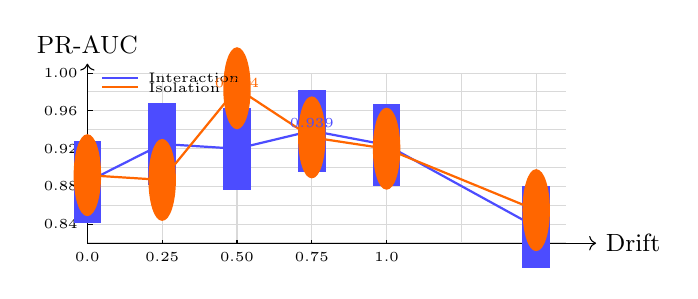
\begin{tikzpicture}[xscale=3.8, yscale=12]
  % Grid
  \draw[gray!30, thin] (0, 0.82) grid[xstep=0.25, ystep=0.02] (1.6, 1.0);
  \draw[->] (0, 0.82) -- (1.7, 0.82) node[right, font=\small] {Drift};
  \draw[->] (0, 0.82) -- (0, 1.01) node[above, font=\small] {PR-AUC};
  % Y-axis labels
  \foreach \y in {0.84, 0.88, 0.92, 0.96, 1.00}
    \draw (0, \y) node[left, font=\tiny] {\y} -- ++(0.02, 0);
  % X-axis labels
  \foreach \x in {0.0, 0.25, 0.50, 0.75, 1.0, 1.5}
    \draw (\x, 0.82) node[below, font=\tiny] {\x} -- ++(0, 0.003);
  % Interaction line (blue)
  \draw[blue!70, thick, mark=square*, mark size=1.2pt]
    plot coordinates {(0.0, 0.885) (0.25, 0.925) (0.50, 0.920)
    (0.75, 0.939) (1.0, 0.924) (1.5, 0.837)};
  % Isolation line (orange)
  \draw[orange!80!red, thick, mark=*, mark size=1.2pt]
    plot coordinates {(0.0, 0.892) (0.25, 0.887) (0.50, 0.984)
    (0.75, 0.932) (1.0, 0.920) (1.5, 0.855)};
  % Legend
  \draw[blue!70, thick] (0.05, 0.995) -- ++(0.12, 0)
    node[right, font=\tiny, black] {Interaction};
  \draw[orange!80!red, thick] (0.05, 0.985) -- ++(0.12, 0)
    node[right, font=\tiny, black] {Isolation};
  % Annotations
  \node[font=\tiny, orange!80!red] at (0.50, 0.990) {$0.984$};
  \node[font=\tiny, blue!70] at (0.75, 0.947) {$0.939$};
\end{tikzpicture}
\caption{The isolation-interaction tradeoff across drift strengths.
Isolation mode peaks at drift${}=0.50$ where the temporal view provides
a near-perfect signal; interaction mode excels at drift${}=0.75$--$1.0$
where cross-view reinforcement is critical.
Neither mode dominates, confirming Proposition~\ref{prop:mode_selection}.}
\label{fig:isolation}
\end{figure}

% ---- 5.3 Observer Ablation ----
\subsection{Geometric Observers are Essential}
\label{sec:observer_analysis}

The strongest evidence for geometric perception as a routing prior comes
from observer ablation (\Cref{tab:observer_analysis}).

\begin{table}[t]
\centering
\caption{Observer ablation (zeroing each family, drift${}=0.75$,
interaction mode, baseline PR-AUC = 0.939).}
\label{tab:observer_analysis}
\begin{tabular}{@{}lcc@{}}
\toprule
Ablation & PR-AUC & $\Delta$ \\
\midrule
No curvature & 0.864 & $-7.5\%$ \\
No view degrees & 0.879 & $-6.0\%$ \\
No LID+curvature+LOF & 0.854 & $-8.6\%$ \\
No LOF & 0.925 & $-1.4\%$ \\
No LID & 0.929 & $-1.1\%$ \\
No diffusion coordinates & 0.935 & $-0.5\%$ \\
No kNN statistics & 0.936 & $-0.3\%$ \\
\bottomrule
\end{tabular}
\end{table}

\textbf{Curvature is the single most critical observer} ($-7.5\%$),
exceeding the impact of removing network depth ($-5.9\%$,
\Cref{tab:ablation}) or the MoE routing mechanism itself ($-2.4\%$).
This ordering is noteworthy: it implies that the \emph{quality} of the
routing signal (from curvature) matters more than the \emph{mechanism}
of routing (sparse top-$k$ selection), validating the central claim
that geometric structure carries irreplaceable routing information.
Removing all three geometric observers (LID, curvature, LOF) together
causes $-8.6\%$---comparable to removing the entire multi-view routing
mechanism.

Observer non-redundancy is confirmed by PCA analysis: the effective
rank is 19.95 out of 64 features, with only 2.8\% of feature pairs
exceeding $|r| > 0.8$.
\Cref{fig:observer_ablation} visualizes the ablation.

\begin{figure}[t]
\centering
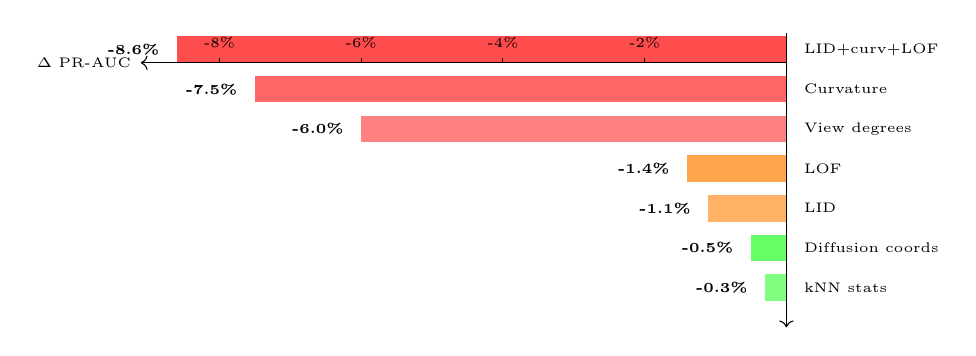
\begin{tikzpicture}[xscale=1, yscale=0.42]
  % Bars (horizontal, sorted by impact)
  \def\bardata{
    {LID+curv+LOF/-8.6/red!70},
    {Curvature/-7.5/red!60},
    {View degrees/-6.0/red!50},
    {LOF/-1.4/orange!70},
    {LID/-1.1/orange!60},
    {Diffusion coords/-0.5/green!60},
    {kNN stats/-0.3/green!50}%
  }
  \foreach \name/\val/\col [count=\i from 0] in \bardata {
    \fill[\col] (0, -\i*1.2) rectangle (\val*0.9, -\i*1.2+0.8);
    \node[right, font=\tiny] at (0.1, -\i*1.2+0.4) {\name};
    \node[left, font=\tiny\bfseries] at (\val*0.9-0.1, -\i*1.2+0.4) {\val\%};
  }
  % Axis
  \draw[->] (0, 0.9) -- (0, -8.0);
  \draw[->] (0, 0) -- (-8.2, 0) node[left, font=\tiny] {$\Delta$ PR-AUC};
  \foreach \x in {-2, -4, -6, -8}
    \draw (\x*0.9, 0) -- ++(0, 0.15) node[above, font=\tiny] {\x\%};
\end{tikzpicture}
\caption{Observer feature ablation (drift${}=0.75$, interaction mode).
Curvature ($-7.5\%$) and view degrees ($-6.0\%$) are the most critical.
Removing all three geometric observers together ($-8.6\%$) is
comparable to removing the entire multi-view routing mechanism.}
\label{fig:observer_ablation}
\end{figure}

% ---- 5.4 Component Ablation ----
\subsection{Component Ablation}
\label{sec:ablation_components}

\begin{table}[t]
\centering
\caption{Component ablation from full \ours{} (interaction mode,
drift${}=0.75$, PR-AUC = 0.939).}
\label{tab:ablation}
\begin{tabular}{@{}lcc@{}}
\toprule
Configuration & PR-AUC & $\Delta$ \\
\midrule
Full \ours{} & 0.939 & --- \\
No depth (1 layer) & 0.880 & $-5.9\%$ \\
No MoE (dense softmax) & 0.915 & $-2.4\%$ \\
No FGW alignment & 0.927 & $-1.2\%$ \\
Single-scale diffusion & 0.936 & $-0.3\%$ \\
\bottomrule
\end{tabular}
\end{table}

\Cref{tab:baselines} shows that \ours{} outperforms GAT by
2.0 points and the best single-view model (diffusion) by 0.9 points.
Uniform multi-view mixing matches GAT, confirming that
\emph{learned routing}---not merely multi-view availability---drives
the gain.

\begin{table}[t]
\centering
\caption{Full model comparison at drift${}=0.75$.}
\label{tab:baselines}
\begin{tabular}{@{}lc@{}}
\toprule
Model & PR-AUC \\
\midrule
\ours{} (interaction, full) & \textbf{0.939} \\
Single-view: diffusion & 0.930 \\
Single-view: $k$NN & 0.923 \\
Router, no alignment & 0.921 \\
GAT \citep{velickovic2018graph} & 0.919 \\
Uniform multi-view & 0.919 \\
\ours{}, no MoE & 0.915 \\
Single-view: temporal & 0.887 \\
\ours{}, no depth & 0.880 \\
\bottomrule
\end{tabular}
\end{table}

% ---- 5.5 Routing Analysis ----
\subsection{Routing Analysis}
\label{sec:routing_analysis}

\begin{table}[t]
\centering
\caption{Learned routing probabilities per head (top-$k=2$,
drift${}=0.75$). Heads specialize on distinct view pairs.}
\label{tab:routing}
\begin{tabular}{@{}lcccl@{}}
\toprule
Head & kNN & Time & Diffusion & Specialization \\
\midrule
0 & 0.347 & 0.072 & 0.580 & Geometry \\
1 & 0.812 & 0.000 & 0.188 & Feature \\
2 & 0.126 & 0.874 & 0.000 & Temporal \\
3 & 0.053 & 0.224 & 0.723 & Diffusion \\
\bottomrule
\end{tabular}
\end{table}

Only 1 of 4 heads specializes on temporal proximity, despite temporal
being the strongest individual signal.
The router distributes capacity across views---suboptimal when one view
dominates, but optimal for complementary regimes.
Top-$k$ sweep: $k=1$ yields 0.931, $k=2$ yields 0.939 (optimal),
$k=3$ yields 0.926.

% ---- 5.6 Stability ----
\subsection{Log-Barrier Stability}
\label{sec:stability}

\begin{table}[t]
\centering
\caption{Adaptive temperature $\tau_h$ recovery under normalization
(drift${}=0.75$, interaction mode).}
\label{tab:stability}
\begin{tabular}{@{}lcccc@{}}
\toprule
Normalization & Baseline & $+\tau_h$ & $\Delta$ & Recovery \\
\midrule
None (default) & 0.939 & 0.943 & $+0.3\%$ & --- \\
Symmetric & 0.937 & 0.936 & $-0.1\%$ & --- \\
Row & 0.923 & 0.929 & $+0.6\%$ & 37\% \\
Self-loops & 0.852 & 0.894 & $+4.2\%$ & 48\% \\
\bottomrule
\end{tabular}
\end{table}

The adaptive temperature provides the greatest benefit where
normalization is most destructive: 48\% recovery under self-loops,
37\% under row normalization.
Self-loops harm performance ($-8.7\%$) because the pre-norm residual
connections already preserve self-information.

% ---- 5.7 Negative Results ----
\subsection{Negative Results: Capacity vs.\ Bottleneck}
\label{sec:thornpp_eval}

\begin{table}[t]
\centering
\caption{Extended model (\ourspp{}) evaluation. View-specific
projections degrade at current scale; online proxy is competitive
only in isolation mode.}
\label{tab:thornpp}
\begin{tabular}{@{}lccc@{}}
\toprule
Configuration & PR-AUC & $\Delta$ & Notes \\
\midrule
\multicolumn{4}{@{}l}{\emph{Isolation mode, drift${}=0.50$}} \\
\ours{} (baseline) & 0.984 & --- & FGW, shared $Q/K/V$ \\
$+$ view-specific $Q/K/V$ & 0.954 & $-3.0\%$ & overfitting \\
$+$ online proxy (no FGW) & 0.984 & $+0.0\%$ & $O(E)$ \\
\midrule
\multicolumn{4}{@{}l}{\emph{Interaction mode, drift${}=0.75$}} \\
\ours{} (baseline) & 0.939 & --- & FGW, shared $Q/K/V$ \\
$+$ adaptive $\tau_h$ & 0.943 & $+0.3\%$ & calibration \\
$+$ online proxy (no FGW) & 0.893 & $-4.7\%$ & misses structure \\
\bottomrule
\end{tabular}
\end{table}

These results illustrate a general architectural principle:
\textbf{capacity added to a non-bottleneck component is
counterproductive}.
At 512 nodes with 3 views sharing the same feature space, the
bottleneck is view selection (routing), not per-view attention
computation.
LoRA-style view-specific projections add capacity to the latter and
degrade by 3--6\%.
The online alignment proxy matches FGW in isolation mode (where
cross-view consensus matters less) but loses 4.7\% in interaction mode,
where edge-level structural agreement is essential.
Only the adaptive temperature $\tau_h$ provides a universal benefit,
confirming its role as a calibration mechanism rather than a capacity
increase.


% ============================================================
%  6. PRACTITIONER'S GUIDE
% ============================================================
\section{Practitioner's Guide: Choosing the Attention Mode}
\label{sec:guide}

The isolation-interaction tradeoff is a first-class hyperparameter.
We provide a decision framework based on two measurable properties of
the available views:

\paragraph{Step 1: Estimate view quality disparity.}
For each view $m$, estimate the task-relevant signal quality (e.g., via
a simple single-view classifier on a validation set, or by computing
within-view label homophily).
If one view's quality dramatically exceeds others, use
\textbf{isolation mode}.

\paragraph{Step 2: Measure view overlap.}
Compute the Jaccard overlap
$\rho = |\calN^{(a)} \cap \calN^{(b)}| / |\calN^{(a)} \cup \calN^{(b)}|$
across view pairs.
High overlap ($\rho > 0.3$) with comparable view quality suggests
\textbf{interaction mode}---cross-view reinforcement is available and
worth exploiting.

\paragraph{Step 3: Check for regime shifts.}
If the data is non-stationary (temporal drift, concept drift),
interaction mode is more robust: it can discover that edges supported by
multiple views are more trustworthy across regimes.
Isolation mode risks locking onto a view that becomes unreliable after
a shift.

\paragraph{Summary rule of thumb.}
\begin{center}
\begin{tabular}{@{}lcl@{}}
\toprule
Signal structure & Overlap & Recommended mode \\
\midrule
One view dominates & Any & Isolation \\
Views comparable, high overlap & $\rho > 0.3$ & Interaction \\
Views comparable, low overlap & $\rho < 0.3$ & Either (tune) \\
Non-stationary data & Any & Interaction \\
\bottomrule
\end{tabular}
\end{center}

When uncertain, treat the mode as a hyperparameter and select via
validation performance---our experiments show that the gap between modes
can exceed 6 PR-AUC points.


% ============================================================
%  7. DISCUSSION
% ============================================================
\section{Discussion}
\label{sec:discussion}

\paragraph{Why geometric descriptors outperform content features for routing.}
The observer ablation (\Cref{sec:observer_analysis}) provides direct
evidence: curvature alone accounts for 7.5\% of performance---more than
the entire MoE routing mechanism (2.4\%) or FGW alignment (1.2\%).
This asymmetry has a structural explanation.
Content-based routers must learn view-relevance associations from
scratch via backpropagation through the task loss.
Geometric observers, by contrast, encode manifold structure
\emph{directly}: curvature reveals bottlenecks where information flow
is constrained, LID reveals dimensionality transitions between dense
clusters and sparse boundaries, and LOF reveals density anomalies that
distinguish normal from atypical connectivity.
This structural prior accelerates routing convergence and yields more
interpretable head specialization (\Cref{tab:routing}).

\paragraph{Generality of the isolation-interaction tradeoff.}
The tradeoff formalized in \Cref{sec:tradeoff} is not specific to
graphs.
Any architecture combining multiple information sources---multi-modal
transformers fusing vision and language, ensemble methods aggregating
base learners, multi-resolution networks processing features at
different scales---faces the same choice: should sources interact
before or after normalization?
Our formalization via $\mathrm{SNR}_m$ and $\rho_i$
(Proposition~\ref{prop:mode_selection}) and the practitioner's guide
(\Cref{sec:guide}) provide, to our knowledge, the first formal
treatment and practical decision framework for this phenomenon in the
attention literature.

\paragraph{When more capacity hurts.}
The negative results in \Cref{sec:thornpp_eval} illustrate a broader
principle: architectural capacity is beneficial only when it targets the
actual bottleneck.
At 512 nodes with views sharing the same feature space, the bottleneck
is in \emph{which view to attend to} (routing), not in \emph{how to
attend within each view} (projection).
Adding LoRA-style view-specific projections adds capacity to the
non-bottleneck component and degrades performance by 3--6\%.
This finding echoes the ``bitter lesson'' in reverse: sometimes the
right inductive bias (geometric routing) outperforms adding parameters.

\paragraph{Connection to geometric deep learning.}
\ours{} contributes to the geometric deep learning program from a new
angle.
Curvature-based graph rewiring \citep{topping2022understanding}
modifies graph \emph{structure} to address over-squashing; \ours{} uses
curvature to modify \emph{attention flow} over a fixed structure.
These are complementary---rewiring changes the graph, routing changes
how information propagates on it---and a natural extension combines
both.


% ============================================================
%  8. CONCLUSION
% ============================================================
\section{Conclusion}
\label{sec:conclusion}

We have identified and formalized a fundamental isolation-interaction
tradeoff in multi-view graph attention: no single mixing mode dominates,
and the optimal choice is predictable from measurable view properties.
Geometric observer routing (\ours{}) exploits this tradeoff by using
manifold descriptors---curvature, intrinsic dimension, density---to
inform view selection, achieving 0.984~PR-AUC in isolation mode (+6.5
over GAT) and 0.939 in interaction mode (+2.0) on a controlled
benchmark.
The ablation evidence is unambiguous: curvature alone carries more
routing signal ($-7.5\%$) than the entire MoE mechanism ($-2.4\%$),
validating geometric descriptors as a principled basis for
attention routing.

\paragraph{Limitations.}
Our evaluation uses a synthetic 512-node benchmark with single-seed
results; scalability to real-world graphs (OGB, heterogeneous knowledge
graphs) and multi-seed statistical validation are essential next steps.
Observer features are computed offline and not updated during training.
The \ourspp{} extensions degrade at current scale, suggesting the
architecture is at a capacity plateau for this benchmark.

\paragraph{Future directions.}
Three extensions are particularly promising:
(1)~\emph{Large-scale evaluation} on real-world benchmarks to test
whether the mechanistic findings generalize beyond synthetic data.
(2)~\emph{Per-head mode selection}: allowing each head to independently
choose isolation or interaction via a learned gate, capturing both
within a single forward pass.
(3)~\emph{Adaptive regime detection}: automatically detecting when the
view correlation structure shifts and adjusting the mode accordingly,
enabling deployment on non-stationary graphs.

% ============================================================
%  REFERENCES
% ============================================================
\bibliographystyle{plainnat}
\bibliography{references}

\end{document}
